\subsubsection{x86: 3つの引数}
% to be sync: \subsubsection{x86: 3 integer arguments}

\myparagraph{MSVC}

MSVC 2010 Expressでコンパイルすると、

\begin{lstlisting}[style=customasmx86]
$SG3830	DB	'a=%d; b=%d; c=%d', 00H

...

	push	3
	push	2
	push	1
	push	OFFSET $SG3830
	call	_printf
	add	esp, 16					; 00000010H
\end{lstlisting}

ほぼ同じですが、 \printf の引数が逆の順序でスタックにプッシュされるのが分かります。 最初の引数は最後にプッシュされます。

ちなみに、32ビット環境での \Tint 型の変数は、32ビット幅、つまり4バイトです。

だから、ここでは4つの引数があります。 $4*4 = 16$。スタック内でちょうど16バイトを占める:文字列への32ビットポインタと \Tint 型の3つの数字。

\myindex{x86!\Instructions!ADD}
\myindex{x86!\Registers!ESP}
\myindex{cdecl}
\gls{stack pointer}(\ESP レジスタ)が関数呼び出しの後の\INS{ADD ESP, X}命令によって元の状態に戻ったとき、関数引数の数はXを4で割るするだけで推測できます。

もちろん、これは\emph{cdecl}呼び出し規約に固有のものであり、32ビット環境のみに適用されます。 

呼び出し規約を参照してください。~(\myref{sec:callingconventions})

いくつかの関数が互いに直後に戻る特定のケースでは、コンパイラは最後の呼び出しの後に複数の \q{ADD ESP, X}命令を1つにマージすることができます:

\begin{lstlisting}[style=customasmx86]
push a1
push a2
call ...
...
push a1
call ...
...
push a1
push a2
push a3
call ...
add esp, 24
\end{lstlisting}

実際の例がここにあります。

\lstinputlisting[caption=x86,style=customasmx86]{patterns/03_printf/x86/add_example_JA.lst}

\clearpage
\myparagraph{MSVC と \olly}
\myindex{\olly}

では、この例を \olly に読み込みましょう。 
これは最もポピュラーなユーザーランドwin32デバッガーの1つです。 
MSVC 2012で\GTT{/MD}オプションを使用してサンプルをコンパイルすることができます。
これは\GTT{MSVCR*.DLL}とリンクすることを意味し、インポートされた関数をデバッガではっきりと見ることができます。

その後、 \olly で実行可能ファイルをロードします。 
最初のブレークポイントは\GTT{ntdll.dll}にあり、
F9(実行)を押します。 
2番目のブレークポイントは\ac{CRT}コードです。 
\main 関数を見つけなければなりません。

コードを一番上までスクロールしてコードを見つけます(MSVCはコードセクションの最初のところで \main 関数を割り当てます)。
\begin{figure}[H]
\centering
\myincludegraphics{patterns/03_printf/x86/olly3_1.png}
\caption{\olly: the very start of the \main function}
\label{fig:printf3_olly_1}
\end{figure}

\INS{PUSH EBP}命令をクリックし、F2(ブレークポイントを設定)を押し、F9(実行)を押します。 
\ac{CRT}コードをスキップするためには、これらの処理を実行する必要があります。なぜなら、実際にはまだ興味がないからです。

\clearpage
F8(\stepover)を6回押します、つまり6つの命令をスキップします。

\begin{figure}[H]
\centering
\myincludegraphics{patterns/03_printf/x86/olly3_2.png}
\caption{\olly: before \printf execution}
\label{fig:printf3_olly_2}
\end{figure}

これで、\ac{PC}は\INS{CALL printf}命令を指し示します。 
\olly は他のデバッガと同様に、変更されたレジスタの値を強調表示します。 
したがって、F8を押すたびに \EIP が変化し、その値が赤で表示されます。 
引数の値がスタックにプッシュされるため、 \ESP も変更されます。

スタック内の値はどこにありますか? 
右下のデバッガーウィンドウを見てみましょう:

\begin{figure}[H]
\centering
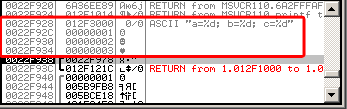
\includegraphics[width=0.5\textwidth]{patterns/03_printf/x86/olly3_stack.png}

\caption{\olly :引数の値がプッシュされた後のスタック(赤い長方形の枠線はグラフィックエディタで作者によって追加されました)}
\end{figure}

スタック内のアドレス、スタック内の値、および追加の \olly コメントが3つあります。 
\olly は \printf のような文字列を理解しているので、ここに文字列とそれに\emph{付随する}3つの値を報告します。
% to be sync: \olly can detect pointers to ASCII strings in stack, so it reports the \printf{}-string here.

フォーマット文字列を右クリックし、\q{Follow in dump}をクリックすると、
フォーマット文字列がデバッガの左下のウィンドウに表示され、メモリの一部が常に表示されます。 
これらのメモリ値は編集できます。 
書式文字列を変更することができます。この場合、例の結果は異なります。 
この特殊なケースではそれほど有用ではありませんが、エクササイズとしてはいいかもしれません。

\clearpage
F8キーを押します(ステップオーバー)。

コンソールに次の出力が表示されます。

\lstinputlisting{patterns/03_printf/x86/console.txt}

レジスタとスタックの状態がどのように変化したかを見てみましょう。

\begin{figure}[H]
\centering
\myincludegraphics{patterns/03_printf/x86/olly3_3.png}
\caption{\printf{} 実行後の \olly }
\label{fig:printf3_olly_3}
\end{figure}

レジスタ \EAX に\GTT{0xD}(13)が含まれるようになりました。 
\printf は印刷された文字数を返すので正しい。 
\EIP の値は変更されました。実際、\INS{CALL printf}の後に来る命令のアドレスを含んでいます。 
\ECX と \EDX の値も変更されています。 
明らかに、 \printf 関数の隠れた機構は、自身の必要のため、それらを使用しました。

非常に重要な事実は、 \ESP 値もスタック状態も変更されていないことです!
フォーマット文字列とそれに対応する3つの値がまだ存在することがわかります。
実際には、これは\emph{cdecl}呼び出し規約の動作です:\gls{callee}は \ESP を以前の値に戻しません。 
\gls{caller}はこれを行う責任があります。

\clearpage
F8をもう一度押して\INS{ADD ESP, 10}命令を実行します。

\begin{figure}[H]
\centering
\myincludegraphics{patterns/03_printf/x86/olly3_4.png}
\caption{\INS{ADD ESP, 10}命令実行後の \olly }
\label{fig:printf3_olly_4}
\end{figure}

\ESP は変更されましたが、値はまだスタックにあります! 
はい、もちろん; これらの値をゼロなどに設定する必要はありません。 
スタックポインタ(\ac{SP})の上にあるものは
すべて\emph{ノイズ}や\emph{\garbage{}}であり、まったく意味がありません。
とにかく、未使用のスタックエントリをクリアするのに時間がかかり、誰も本当に必要とはしません。

\myparagraph{GCC}
GCC 4.4.1を使って同じプログラムをLinuxでコンパイルして、 \IDA で何が得られたかを見てみましょう。

\lstinputlisting[style=customasmx86]{patterns/03_printf/x86/x86_1.asm}

MSVCコードとGCCコードの違いは、引数がスタックに格納される方法だけにあることに注目してください。 
ここでGCCは \PUSH/\POP を使用せずに、スタックを直接使用してスタックを操作しています

\myparagraph{GCC and GDB}
\myindex{GDB}

Linuxの\ac{GDB}でもこの例を試してみましょう。

\GTT{-g}オプションは、デバッグ情報を実行可能ファイルに含めるようにコンパイラに指示します。

\begin{lstlisting}
$ gcc 1.c -g -o 1
\end{lstlisting}

\begin{lstlisting}
$ gdb 1
GNU gdb (GDB) 7.6.1-ubuntu
...
Reading symbols from /home/dennis/polygon/1...done.
\end{lstlisting}

\begin{lstlisting}[caption= \printf にブレークポイントを設定しましょう]
(gdb) b printf
Breakpoint 1 at 0x80482f0
\end{lstlisting}

実行します。
ここには \printf 関数のソースコードがありませんので、\ac{GDB}はそれを表示することはできませんが、実行することはできます。

\begin{lstlisting}
(gdb) run
Starting program: /home/dennis/polygon/1 

Breakpoint 1, __printf (format=0x80484f0 "a=%d; b=%d; c=%d") at printf.c:29
29	printf.c: No such file or directory.
\end{lstlisting}

スタック要素を10個表示します。 最も左の列には、スタック上のアドレスが含まれています。

\begin{lstlisting}
(gdb) x/10w $esp
0xbffff11c:	0x0804844a	0x080484f0	0x00000001	0x00000002
0xbffff12c:	0x00000003	0x08048460	0x00000000	0x00000000
0xbffff13c:	0xb7e29905	0x00000001
\end{lstlisting}

最初の要素は\ac{RA}(\GTT{0x0804844a})です。 
このアドレスのメモリを逆アセンブルして確認することができます:

\begin{lstlisting}[label=NOP_as_XCHG_example,style=customasmx86]
(gdb) x/5i 0x0804844a
   0x804844a <main+45>:	mov    $0x0,%eax
   0x804844f <main+50>:	leave  
   0x8048450 <main+51>:	ret    
   0x8048451:	xchg   %ax,%ax
   0x8048453:	xchg   %ax,%ax
\end{lstlisting}

2つの\INS{XCHG}命令は、\ac{NOP}に類似したアイドル命令です。

2番目の要素(\GTT{0x080484f0})はフォーマット文字列アドレスです。

\begin{lstlisting}
(gdb) x/s 0x080484f0
0x80484f0:	"a=%d; b=%d; c=%d"
\end{lstlisting}

次の3つの要素(1,2,3)は \printf の引数です。
残りの要素はスタック上の \q{garbage}に過ぎないかもしれませんが、
他の関数やローカル変数などからの値であってもかまいません。

\q{finish}を実行します。 
このコマンドは、GDBに\q{関数の最後まですべての命令を実行する}よう指示します。 
この場合、 \printf の最後まで実行してください。

\begin{lstlisting}
(gdb) finish
Run till exit from #0  __printf (format=0x80484f0 "a=%d; b=%d; c=%d") at printf.c:29
main () at 1.c:6
6		return 0;
Value returned is $2 = 13
\end{lstlisting}

\ac{GDB}は、\printf が \EAX (13)をリターンしたことを示しています。 
これは、 \olly の例のように、印刷される文字の数です。

また、 \q{return 0;}と、この式が6行目の\GTT{1.c}ファイルにあるという情報も表示されます。
実際には、\GTT{1.c}ファイルは現在のディレクトリにあり、\ac{GDB}はその文字列を見つけます。 
どのCコード行が現在実行されているかを\ac{GDB}はどうやってに知るのでしょうか?
これは、コンパイラがデバッグ情報を生成している間に、
ソースコードの行番号と命令アドレスの間の関係のテーブルも保存しているためです。 
GDBはソースレベルのデバッガです。

レジスタを調べてみましょう。 
EAXには13が入っています

\begin{lstlisting}
(gdb) info registers
eax            0xd	13
ecx            0x0	0
edx            0x0	0
ebx            0xb7fc0000	-1208221696
esp            0xbffff120	0xbffff120
ebp            0xbffff138	0xbffff138
esi            0x0	0
edi            0x0	0
eip            0x804844a	0x804844a <main+45>
...
\end{lstlisting}

現在の命令を逆アセンブルしましょう。
矢印は、次に実行される命令を指し示します。

\begin{lstlisting}[style=customasmx86]
(gdb) disas
Dump of assembler code for function main:
   0x0804841d <+0>:	push   %ebp
   0x0804841e <+1>:	mov    %esp,%ebp
   0x08048420 <+3>:	and    $0xfffffff0,%esp
   0x08048423 <+6>:	sub    $0x10,%esp
   0x08048426 <+9>:	movl   $0x3,0xc(%esp)
   0x0804842e <+17>:	movl   $0x2,0x8(%esp)
   0x08048436 <+25>:	movl   $0x1,0x4(%esp)
   0x0804843e <+33>:	movl   $0x80484f0,(%esp)
   0x08048445 <+40>:	call   0x80482f0 <printf@plt>
=> 0x0804844a <+45>:	mov    $0x0,%eax
   0x0804844f <+50>:	leave  
   0x08048450 <+51>:	ret    
End of assembler dump.
\end{lstlisting}

\ac{GDB}はデフォルトでAT\&T構文を使用します。
しかし、インテルの構文に切り替えることは可能です:

\begin{lstlisting}[style=customasmx86]
(gdb) set disassembly-flavor intel
(gdb) disas
Dump of assembler code for function main:
   0x0804841d <+0>:	push   ebp
   0x0804841e <+1>:	mov    ebp,esp
   0x08048420 <+3>:	and    esp,0xfffffff0
   0x08048423 <+6>:	sub    esp,0x10
   0x08048426 <+9>:	mov    DWORD PTR [esp+0xc],0x3
   0x0804842e <+17>:	mov    DWORD PTR [esp+0x8],0x2
   0x08048436 <+25>:	mov    DWORD PTR [esp+0x4],0x1
   0x0804843e <+33>:	mov    DWORD PTR [esp],0x80484f0
   0x08048445 <+40>:	call   0x80482f0 <printf@plt>
=> 0x0804844a <+45>:	mov    eax,0x0
   0x0804844f <+50>:	leave  
   0x08048450 <+51>:	ret    
End of assembler dump.
\end{lstlisting}

次の命令を実行します。 
% to be sync: Execute next line of \CCpp{} code.
\ac{GDB}は、終わりの括弧を示します。つまり、ブロックを終了します。

\begin{lstlisting}
(gdb) step
7	};
\end{lstlisting}

\INS{MOV EAX, 0}命令実行後のレジスタを調べてみましょう。 
実際、 \EAX はその時点で0です。

\begin{lstlisting}
(gdb) info registers
eax            0x0	0
ecx            0x0	0
edx            0x0	0
ebx            0xb7fc0000	-1208221696
esp            0xbffff120	0xbffff120
ebp            0xbffff138	0xbffff138
esi            0x0	0
edi            0x0	0
eip            0x804844f	0x804844f <main+50>
...
\end{lstlisting}

